\documentclass[conference]{IEEEtran}

\usepackage{cite}
\usepackage{amsmath}
\usepackage{amssymb}
\usepackage{url}
\usepackage{graphicx}
\usepackage{booktabs}
\usepackage{microtype}
\usepackage[table]{xcolor}
\usepackage{tikz}
\usetikzlibrary{positioning,arrows.meta}
\usepackage{pgfplots}
\pgfplotsset{compat=1.18}
\usepgfplotslibrary{groupplots}
\usepackage[hidelinks]{hyperref}

\definecolor{phaseblue}{RGB}{52,152,219}
\definecolor{phasegreen}{RGB}{46,204,113}
\definecolor{phaseorange}{RGB}{230,126,34}
\definecolor{phasepurple}{RGB}{155,89,182}

\title{{\LARGE\textbf{A Reproducible Framework for Fairness-Aware Contextual Bandits Under Missing Context}}\\
{\Large\textit{Quantum Routing Evidence and a Planned Diagnostic Simulator}}\\[0.25em]
{\large\textit{(draft1 revision of the rough draft report)}}}

\author{
\IEEEauthorblockN{Piter Z. Garcia}
\IEEEauthorblockA{MS Data Science / Decision-Making \& Algorithmic Fairness\\
Rochester Institute of Technology (RIT)\\
pizg8794@g.rit.edu}
\and
\IEEEauthorblockN{Daniel Krutz, Travis Desell}
\IEEEauthorblockA{Department of Software Engineering, Data Science\\
Rochester Institute of Technology (RIT)\\
dxkvse@g.rit.edu, tjdvse@g.rit.edu}
}

\begin{document}
\maketitle

\begin{abstract}
This paper studies fairness-aware sequential decision making under missing, delayed, noisy, or group-dependent context. The central claim is that incomplete context is not only a modeling inconvenience; it can also become a mechanism for repeated allocation inequity in partial-feedback systems. The project is motivated by two domains with the same structural problem: quantum entanglement routing and diagnostic decision workflows. In both cases, a policy observes imperfect context, selects among limited actions, and receives feedback only on the chosen action. The current evidence base is strongest on the quantum side, where inherited routing corpora and documented execution paths already provide realistic utility and robustness evidence. The clinical side remains simulation-first and is framed here as the next empirical testbed rather than a completed experiment. The contribution of the current phase is therefore a reproducible framework, a clearer cross-domain problem formulation, and a staged plan for measuring utility--fairness tradeoffs under shared evaluation contracts.
\end{abstract}

\section{Introduction}
Many applied data science systems do not make one prediction and stop. They allocate scarce attention, tests, routes, or computational effort repeatedly under uncertainty. Such systems are naturally modeled as sequential decision problems with partial feedback: the learner observes the outcome of the action it chose but not the outcomes of the actions it did not choose. Bandit methods are a natural fit for this structure because they formalize the exploration--exploitation tradeoff while keeping the feedback model realistic~\cite{auer2002finite,russo2018tutorial,lattimore2020bandit}.

This project focuses on a narrower and more consequential question: what happens when context quality is unequal across groups or flows? In diagnostic settings, one subgroup may receive delayed tests, noisier measurements, or less representative calibration data. In quantum routing, one flow class may be served under more uncertain link or load information than another. A policy that optimizes only aggregate reward can then convert unequal context quality into repeated allocation inequity. That mechanism is the conceptual core of the project.

The original rough draft already identified an important cross-domain insight: diagnostic workflows and quantum routing can both be treated as resource-allocation systems under missing context. What needed improvement was scope control. The draft sometimes read like a completed dual-domain fairness study, even though the strongest implemented and evidenced component currently lives on the quantum side, while the clinical side remains a planned simulation-first extension. This revision fixes that mismatch directly.

Accordingly, the paper makes three bounded claims. First, missing context should be treated as part of the scientific problem rather than as an afterthought. Second, fairness evaluation in sequential decision systems should be reported alongside utility and regret, not after them. Third, the present contribution is best understood as a reproducible framework with inherited preliminary quantum evidence and a clear next-step clinical simulator, not as a completed two-domain empirical fairness paper.

\section{Related Work}
Classical stochastic bandits provide the regret and uncertainty machinery that underlies this project~\cite{auer2002finite,russo2018tutorial,lattimore2020bandit}. Contextual bandits extend that setting by conditioning actions on observed side information, enabling stronger personalization and more structured decision making~\cite{li2010contextual,abbasi2011linear,agarwal2014taming}. Offline policy-evaluation work is also relevant because the final framework must compare learned policies from logged trajectories as well as fresh runs~\cite{dudik2011doubly}.

Fairness work adds the second major ingredient. Equality-of-opportunity style metrics formalize group-conditioned error gaps in static supervised settings~\cite{hardt2016equality}. Sequential and bandit-specific fairness research shows that fairness cannot be treated as a simple post-hoc wrapper, because exploration and data collection themselves shape which groups receive evidence and service~\cite{joseph2016fairness,chen2020fair,metevier2019offline}. In parallel, non-stationary bandit work studies changing reward processes through discounting and shift-aware learning~\cite{garivier2008ucb,besbes2014stochastic}, while restricted-context and unobserved-context work studies robustness when side information is incomplete~\cite{bouneffouf2017context,park2022efficient}.

The clinical and quantum literatures motivate the application domains. Clinical bias studies show that measurement processes and proxy targets can encode structural inequity even when headline accuracy looks strong~\cite{obermeyer2019dissecting}. Quantum networking research, by contrast, emphasizes throughput, fidelity, and routing robustness in resource-constrained environments~\cite{wehner2018quantum,pant2019routing,caleffi2017optimal}. The gap is the intersection: prior work rarely studies missing context, non-stationarity, and explicit fairness monitoring together across more than one domain. That joint space is where this project is positioned.

\section{Problem Formulation}
\subsection{Shared missing-context routing model}
The two target domains differ in semantics but share the same decision structure. At round $t$, a learner observes an imperfect context vector $\tilde{\mathbf{x}}_t$, chooses an action $a_t$, and receives reward only for that action. The observed context may differ from the latent full context $\mathbf{x}_t$ because of missingness, delay, or measurement noise. Utility is tracked through cumulative regret,
\begin{equation}
R_T = \sum_{t=1}^{T}\left(r_t(a_t^\star) - r_t(a_t)\right),
\end{equation}
where $a_t^\star$ is the best available action under the simulator oracle. Fairness is tracked through time-indexed disparity,
\begin{equation}
\Delta_m(t) = \left|m_t(G=0)-m_t(G=1)\right|,
\end{equation}
where $m_t$ is a domain-specific outcome metric such as false-negative rate, success probability, or latency.

This formulation matters because it separates two questions that are often conflated. A policy can have low aggregate regret while still producing large subgroup disparity. Conversely, a policy can reduce disparity only by sacrificing too much utility to remain operationally useful. The right scientific target is therefore the utility--fairness tradeoff under changing context quality.

\subsection{Current scope}
The project is intentionally cross-domain, but the evidence is not yet symmetric across domains. The quantum-routing side already has an inherited corpus, documented execution paths, allocator comparisons, and scenario-level result artifacts~\cite{garcia2026threat_aware_quantum_routing}. The clinical side is presently a simulation-first design target informed by earlier fairness-aware bioinformatics work rather than a completed sequential experiment~\cite{garcia2025equitable_bioinformatics}. The report must therefore distinguish \emph{completed evidence}, \emph{partial extensions}, and \emph{planned experiments}.

\begin{table}[t]
\caption{Cross-domain experiment matrix used to define the project cleanly.}
\label{tab:experiment_matrix}
\centering
\small
\begin{tabular}{p{0.18\columnwidth}p{0.19\columnwidth}p{0.19\columnwidth}p{0.34\columnwidth}}
\toprule
\textbf{Domain} & \textbf{Action} & \textbf{Reward} & \textbf{Fairness focus} \\
\midrule
Quantum routing & route / allocator choice & efficiency, success, latency & service-quality gaps across flow classes under unequal context \\
Clinical simulation & test / retest / escalation choice & diagnostic utility, delay, cost & false-negative, false-positive, or delay gaps across protected groups \\
\bottomrule
\end{tabular}
\end{table}

\begin{figure}[t]
\centering
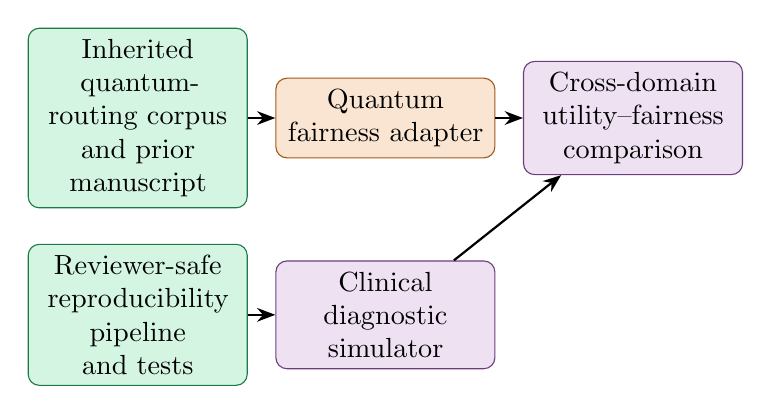
\begin{tikzpicture}[
node distance=0.45cm and 0.35cm,
box/.style={draw, rounded corners=4pt, align=center, minimum height=0.72cm, text width=2.5cm, inner sep=4pt},
done/.style={box, fill=phasegreen!20, draw=phasegreen!60!black},
partial/.style={box, fill=phaseorange!20, draw=phaseorange!70!black},
future/.style={box, fill=phasepurple!18, draw=phasepurple!70!black},
arr/.style={-Stealth, thick}
]
\node[done] (q) {Inherited quantum-routing corpus and prior manuscript};
\node[done, below=of q] (r) {Reviewer-safe reproducibility pipeline and tests};
\node[partial, right=of q] (f) {Quantum fairness adapter};
\node[future, right=of r] (c) {Clinical diagnostic simulator};
\node[future, right=of f] (x) {Cross-domain utility--fairness comparison};

\draw[arr] (q) -- (f);
\draw[arr] (r) -- (c);
\draw[arr] (f) -- (x);
\draw[arr] (c) -- (x);
\end{tikzpicture}
\caption{Revised project scope. The strongest current evidence is inherited quantum-routing evidence plus a reproducibility scaffold. The fairness adapter is the immediate next implementation target, while the clinical simulator and cross-domain comparison belong to the next empirical phase.}
\label{fig:scope}
\end{figure}

\section{Implementation and Reproducibility}
The implementation has two distinct evidence paths. The first is a reviewer-safe CRISP+ML pipeline intended for fast validation of dataflow, configuration, artifact contracts, and fairness-oriented evaluation outputs. The second is the larger quantum-routing research path, which supports notebook, local, and cloud execution and provides the inherited preliminary quantum evidence.

This distinction is a strength, not a weakness. The smaller path makes review practical. It allows another reader to inspect stage boundaries, deterministic artifacts, and command-line entry points without depending on long-running quantum experiments. The larger path provides domain realism and a substantive prior evidence base. Together they support a strong reproducibility claim: the project already has an executable scaffold and a realistic upstream environment, even though the full two-domain fairness study is not yet complete.

The paper should therefore describe the current implementation as a \emph{reproducibility scaffold with staged empirical evidence}, not as a fully validated final system. That wording is more accurate and more professional.

\begin{table}[t]
\caption{Evidence status at the draft1 stage.}
\label{tab:evidence_status}
\centering
\small
\begin{tabular}{p{0.28\columnwidth}p{0.16\columnwidth}p{0.42\columnwidth}}
\toprule
\textbf{Component} & \textbf{Status} & \textbf{How it should be described} \\
\midrule
Quantum-routing corpus & Completed & Preliminary inherited evidence supporting next-stage fairness analysis \\
Reviewer-safe pipeline & Completed & Reproducibility scaffold with CLI, artifacts, and tests \\
Unit-test suite & Completed & Repository contains tests and merge-check path; attach logs only when executed \\
Quantum fairness adapter & Partial & Immediate next implementation target \\
Clinical diagnostic simulator & Planned & Simulation-first next testbed \\
Cross-domain fairness results & Planned & Not yet a completed empirical contribution \\
\bottomrule
\end{tabular}
\end{table}

\section{Current Empirical Evidence}
The strongest quantitative evidence available now comes from the inherited quantum-routing work~\cite{garcia2026threat_aware_quantum_routing}. That evidence is already useful, but it must be described precisely. It supports claims about utility, robustness, and the value of richer context. It does not yet support claims about completed cross-domain fairness performance.

\begin{table*}[t]
\caption{Preliminary quantum evidence that can be used now without overclaiming.}
\label{tab:quantum_prelim}
\centering
\small
\begin{tabular}{p{0.18\textwidth}p{0.24\textwidth}p{0.22\textwidth}p{0.26\textwidth}}
\toprule
\textbf{Evidence source} & \textbf{Current quantitative signal} & \textbf{What it shows} & \textbf{How it should be used in this report} \\
\midrule
Threat-aware quantum manuscript & pursuit--neural hybrids outperform no-context baselines by roughly 18--24 percentage points in scenario-aggregated efficiency & richer context materially improves routing utility & motivates fairness-aware extension of the strongest policy families \\
Internal hybrid corpus & \texttt{iCPursuitNeuralUCB} currently has the strongest average internal efficiency (86.13\%) & identifies the leading current utility baseline & treat as inherited prior evidence, not as a completed fairness result \\
Standardized external corpus & 8,060 rows across multiple allocators, scenarios, scales, and routing models & provides breadth across testbeds and threat regimes & use as the basis for later service-equity benchmarking once flow labels and disparity metrics are added \\
Adversarial stress evidence & replay-capacity changes can trigger large efficiency collapses under adaptive adversaries & deployment quality depends on policy and resource setting together & motivates fairness analysis of allocator and capacity choices, not only model choice \\
\bottomrule
\end{tabular}
\end{table*}

The cleanest way to present the current evidence is as a \emph{context-quality finding}. Across the inherited quantum corpora, richer context improves routing performance relative to no-context baselines. That is already scientifically useful because it identifies where the next fairness layer should attach: if context quality moves utility, then unequal context quality is a plausible mechanism for unequal service quality.

\begin{figure*}[t]
\centering
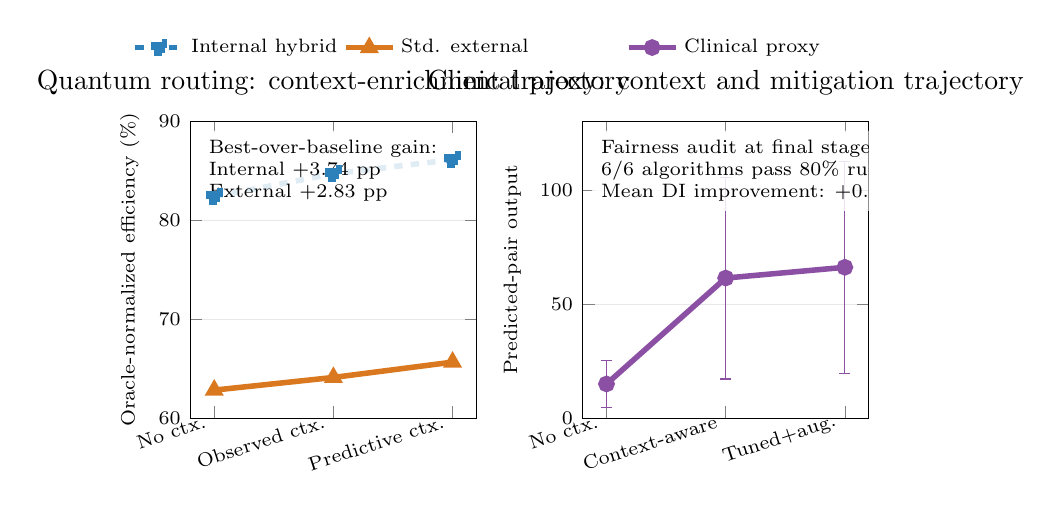
\begin{tikzpicture}
\begin{groupplot}[
group style={group size=2 by 1, horizontal sep=1.35cm},
width=0.43\textwidth,
height=5.35cm,
xtick=data,
xticklabel style={font=\scriptsize, rotate=18, anchor=east},
tick label style={font=\scriptsize},
label style={font=\scriptsize},
ymajorgrids=true,
grid style={line width=.1pt, draw=gray!18},
legend style={font=\scriptsize, draw=none, at={(0.5,1.18)}, anchor=south, legend columns=3},
every axis plot/.append style={line width=2pt},
every mark/.append style={scale=0.9}
]
\nextgroupplot[
title={Quantum routing: context-enrichment trajectory},
ylabel={Oracle-normalized efficiency (\%)},
symbolic x coords={No ctx.,Observed ctx.,Predictive ctx.},
ymin=60, ymax=90
]
\addplot[color=phaseblue!85!black, mark=square*, dashed] coordinates {
  (No ctx.,82.39) (Observed ctx.,84.70) (Predictive ctx.,86.13)
};
\addlegendentry{Internal hybrid}
\addplot[color=phaseorange!95!black, mark=triangle*] coordinates {
  (No ctx.,62.83) (Observed ctx.,64.11) (Predictive ctx.,65.66)
};
\addlegendentry{Std. external}
\node[anchor=north west, font=\scriptsize, align=left,
      fill=white, fill opacity=0.85, text opacity=1, rounded corners=2pt]
  at (rel axis cs:0.03,0.97)
  {Best-over-baseline gain:\\Internal +3.74 pp\\External +2.83 pp};

\nextgroupplot[
title={Clinical proxy: context and mitigation trajectory},
ylabel={Predicted-pair output},
symbolic x coords={No ctx.,Context-aware,Tuned+aug.},
ymin=0, ymax=130
]
\addplot[color=phasepurple!90!black, mark=*, error bars/.cd, y dir=both, y explicit] coordinates {
  (No ctx.,14.96) +- (0,10.45)
  (Context-aware,61.36) +- (0,44.21)
  (Tuned+aug.,66.07) +- (0,46.36)
};
\addlegendentry{Clinical proxy}
\node[anchor=north west, font=\scriptsize, align=left,
      fill=white, fill opacity=0.85, text opacity=1, rounded corners=2pt]
  at (rel axis cs:0.03,0.97)
  {Fairness audit at final stage:\\6/6 algorithms pass 80\% rule\\Mean DI improvement: +0.805};
\end{groupplot}
\end{tikzpicture}
\caption{Cross-testbed context-enrichment trajectories carried forward from the current rough draft. The left panel shows a completed quantum result: routing utility rises monotonically as the policy moves from no context to observed context to predictive context. The right panel shows the role that the clinical proxy currently plays in the evidence stack: it demonstrates a large benefit from restoring domain-relevant context and a smaller later-stage gain from tuning and fairness-aware augmentation, but it remains a motivating evidence package rather than a finished sequential-bandit clinical experiment.}
\label{fig:draft1_context_trajectory}
\end{figure*}

Figure~\ref{fig:draft1_context_trajectory} makes the evidence boundary easier to see. The quantum side already supplies a clean monotone context-enrichment story with inherited empirical support. The clinical side supplies a motivating proxy trajectory and a fairness-audit signal, but not yet a completed diagnostic bandit study. Presenting the evidence this way is both more honest and more persuasive.

The clinical side should be framed more carefully. Prior bioinformatics work supplies a motivating fairness-aware evidence package and helps define what the clinical simulator should measure~\cite{garcia2025equitable_bioinformatics}. It should not be presented as if the diagnostic contextual-bandit experiment has already been implemented end to end. The right wording is that the clinical side is \emph{simulation-first and informed by prior fairness-aware biomedical work}.

\section{Ethics and Validity}
The ethical stakes differ by domain but the design lesson is the same. In diagnostics, missing or low-quality context can produce under-triage, false negatives, or delayed care for some groups. In quantum routing, unequal context quality can degrade service probability or latency for some flows even when average network performance looks acceptable. In both settings, aggregate performance can hide unequal outcomes.

For that reason, fairness in this project is not decorative. It determines what must be logged, how results must be stratified, and how claims should be written. The paper should explicitly distinguish protected groups in the clinical simulator from service classes or flow groups in the quantum domain. That distinction tightens the ethics section and avoids conceptual drift.

There is also a validity issue that should be stated plainly. The current report combines inherited quantum evidence with a planned clinical simulator. The domains are therefore not yet symmetric in implementation maturity. That does not weaken the project. It simply means the present artifact is a framework-and-evidence paper rather than a completed dual-domain comparison.

\section{Next Experimental Phase}
The next phase should be operational, not rhetorical.

First, attach explicit fairness metrics and service-group labels to the quantum corpus. That is the fastest path to a genuine empirical fairness result because the upstream routing data and execution machinery already exist. Second, implement the clinical simulator with controlled missingness, measurement noise, action choices, and protected-group annotations. Third, evaluate at least one mitigation family across both domains: fairness-regularized updates, missingness-aware context augmentation, or group-aware calibration. Fourth, report utility--fairness tradeoff curves under shared evaluation contracts.

This sequence is important. It turns the strongest available evidence into a completed fairness study in one domain before attempting a fully symmetric cross-domain paper. That is the disciplined path.

\section{Conclusion}
The strongest version of this project is not ``we already completed a dual-domain fairness paper.'' The strongest version is more precise: this work establishes a reproducible framework for fairness-aware contextual bandits under missing context, grounded in inherited quantum-routing evidence and extended next by a simulation-first clinical diagnostic testbed.

That framing improves the paper in three ways. It removes vague or inflated wording. It aligns claims with the artifact set that currently exists in the repositories. And it strengthens the scientific story by making the next experimental step obvious. The conceptual contribution remains ambitious, but the evidence boundary is now clear. That is what raises the draft toward a stronger PhD-level standard.

\bibliographystyle{IEEEtran}
\bibliography{../../rough_draft_report/rough_draft_references}

\end{document}